%!TEX root = ../example.tex
%*******************************************************************************
% * Copyright (c) 2006-2013 
% * Institute of Automation, Dresden University of Technology
% * 
% * All rights reserved. This program and the accompanying materials
% * are made available under the terms of the Eclipse Public License v1.0 
% * which accompanies this distribution, and is available at
% * http://www.eclipse.org/legal/epl-v10.html
% * 
% * Contributors:
% *   Institute of Automation - TU Dresden, Germany 
% *      - initial API and implementation
% ******************************************************************************/

%%%%%%%%%%%%%%%%%%%%%%%%%%%%%%%%%%%%%%%%%%%%%%%%%%%%%%%%%%%%%%%%%%%%%%
%%%%%%%%%%%%%%%%%%%%%%%%%%%%%%%%%%%%%%%%%%%%%%%%%%%%%%%%%%%%%%%%%%%%%%
\chapter{Anforderungsdefinition}
\label{sec:AllgemeineHinweiseZurVorlage}

Die Anforderungsspezifikation steht am Anfang des Entwicklungsprozesses. Sie bildet die nötige Grundlage für die Entwicklung eines technischen Systems und ist von großer Bedeutung für den Erfolg dieser Entwicklung.
%%%%%%%%%%%%%%%%%%%%%%%%%%%%%%%%%%%%%%%%%%%%%%%%%%%%%%%%%%%%%%%%%%%%%%

%%%%%%%%%%%%%%%%%%%%%%%%%%%%%%%%%%%%%%%%%%%%%%%%%%%%%%%%%%%%%%%%%%%%%%
\section{Strukturierte Analyse}
%%%%%%%%%%%%%%%%%%%%%%%%%%%%%%%%%%%%%%%%%%%%%%%%%%%%%%%%%%%%%%%%%%%%%%




%%%%%%%%%%%%%%%%%%%%%%%%%%%%%%%%%%%%%%%%%%%%%%%%%
\subsection{Kontextdiagramm}

Ein Kontextdiagramm dient der Modellierung einer Systemumgebung in einer frühen Entwurfs- oder Analysephase.Das Kontextdiagramm stellt die oberste Hierarchieebene von Datenflussdiagrammen dar.Es handelt sich um ein abstraktes Datenflussdiagramm, mit dem die Schnittstellen des Systems zu dessen Umwelt abgebildet werden. Im folgenden Daten- und Steuerkontextdiagramm dieser Arbeit wird das Eingang und Ausgang der Schnittstelle für die Ansteuerung des youBot-Systems bezeichnet, siehe Abbildung 2.1.
Die Tabelle 2.1 beschreibt die angeforderten Datenflüsse.
\begin{figure}[htb]
  \centering
  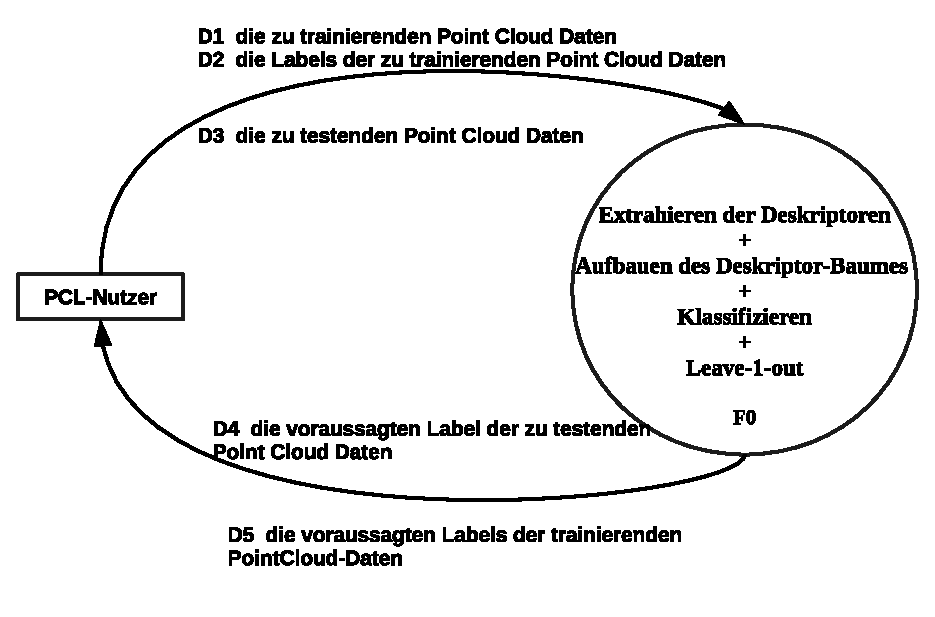
\includegraphics[width=0.7\textwidth]{example_files/log/kontexdiagramm.eps}
  \caption{Kontextdiagramm}\label{fig:digit}

\end{figure}


\begin{table}[h]
\caption{Kontextdiagramm - Daten- und Steuerflüsse}
\centering
\begin{tabular}{p{5.5cm}|p{8cm}}

\hline
\textbf{Datenfluss} & \textbf{Beschreibung}\\
\hline
D1 die zu trainierenden Point Cloud Daten & Die Trainingsdaten im PCD Form, um gute Klassifikatoren zu lernen \\

\hline
D2 die Labels der zu trainierenden Point Cloud Daten  & die Labels für die Trainingsdaten \\
\hline
D3  die zu testenden Point Cloud Daten & Die Testdaten in PCD Form, um die gelernten Klassfikatoren zu testen\\
\hline
D4 die Labels der getesten Point Cloud Daten & die Labels für die getesten Daten , die bei den gelernten Klassifikatoren vorausgesagt werden\\
\hline
D5  die Labels der trainierten Point Cloud Daten & die Labels der Trainingsdaten,  die bei den  gelernten klassifikatoren vorausgesagt werden,  \\
\hline
\end{tabular}
\end{table}

%%%%%%%%%%%%%%%%%%%%%%%%%%%%%%%%%%%%%%%%%%%%%%%%%
\subsection{Datenflussdiagramm - Ebene 1}

Die Aufgabe wird in mehrere Teilaufgaben zerlegt, die Abbildung 2.2 zeigt die
Komposition auf Ebene 1. Die Tabellen 2.2 und 2.3 beschreiben die enthaltenen
Funktionen und Datenflüsse.


\begin{figure}[htb]
  \centering
  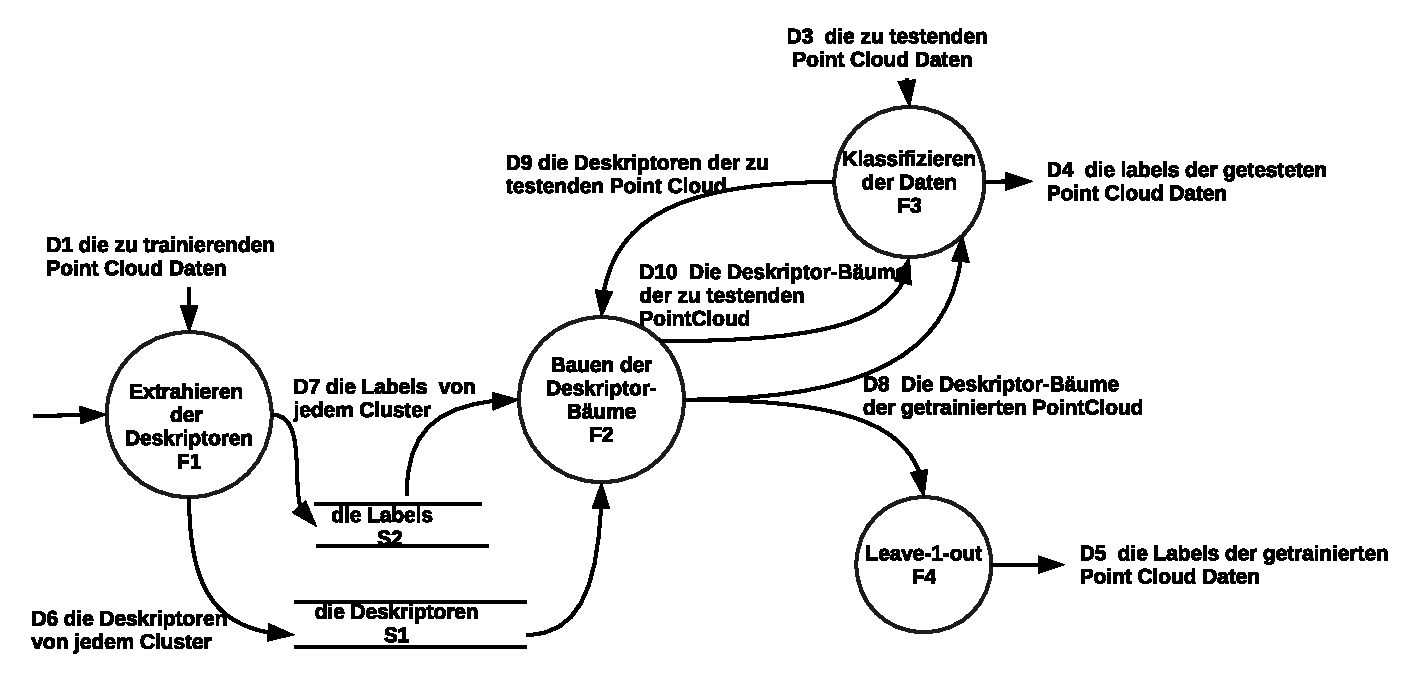
\includegraphics[width=1.0\textwidth]{example_files/log/DE1.eps}
  \caption{Datenflussdiagramm - Ebene 1}\label{fig:digit}
\end{figure}

 \begin{table}[htb]
    \caption{Datenflussdiagramm - Ebene 1 - Funktionen}
     \centering
   \begin{tabular}{p{5.5cm}|p{8cm}}
    \hline
    \textbf{Funktion} & \textbf{Beschreibung}\\
    \hline
     F1  Extrahieren der Deskriptoren& Das Objekt wird in mehrere Cluster unterteilt und die Deskriptoren von jedem Cluster werden berechnet. \\
    \hline
     F2  Bauen des Dekriptor-Baumes &  Der Dekriptor-Baum wird gebaut \\
    \hline
     F3  Klassifizieren der Daten &  
  Die Testdaten werden nach den gelernten Klassifikatoren klassifiziert und erhalten die Prognoselabel    \\
    \hline
     F4  Leave-1-out & die Trainingdaten werden nach den gelernten Klassifkatoren klassifizieren und  erhalten die Prognoselabel\\
    \hline
  \end{tabular}
\end{table}

\begin{table}[htb]
	\caption{Datenflussdiagramm - Ebene 1 - Datenflüsse}
	\centering
	\begin{tabular}{p{5.5cm}|p{8cm}}
		
		\hline
		\textbf{Datenfluss} & \textbf{Beschreibung}\\
		\hline
		D6 die Deskriptoren von jedem Cluster & die Deskriptoren für jeden untergeteilten Cluster \\
		
		\hline
		D7 die Labels  von jedem Cluster  & die Labels für jeden erzeugten Cluster \\
		\hline
		D8  Die Deskriptor-Bäume der getrainierten PointCloud & Die Deskriptor-Bäume von allen Trainingsobjekt\\
		\hline
		D9 die Deskriptoren der zu testenden Point Cloud  & die Deskriptoren für die Test Objekten\\
		\hline
		D10  Die Deskriptor-Bäume der zu testenden PointCloud & Die Deskriptor-Bäume für die Test Objekten  \\
		\hline
	\end{tabular}
\end{table}



%%%%%%%%%%%%%%%%%%%%%%%%%%%%%%%%%%%%%%%%%%%%%%%%%
\subsection{Datenflussdiagramm - Ebene 2 - Funktion 1}

Die im Abschnitt 2.2.2 dargestellten Funtion F1 wird weiter detailliert, um
das Teilsystem deutlich zu machen.

\begin{figure}[h]
    \centering
    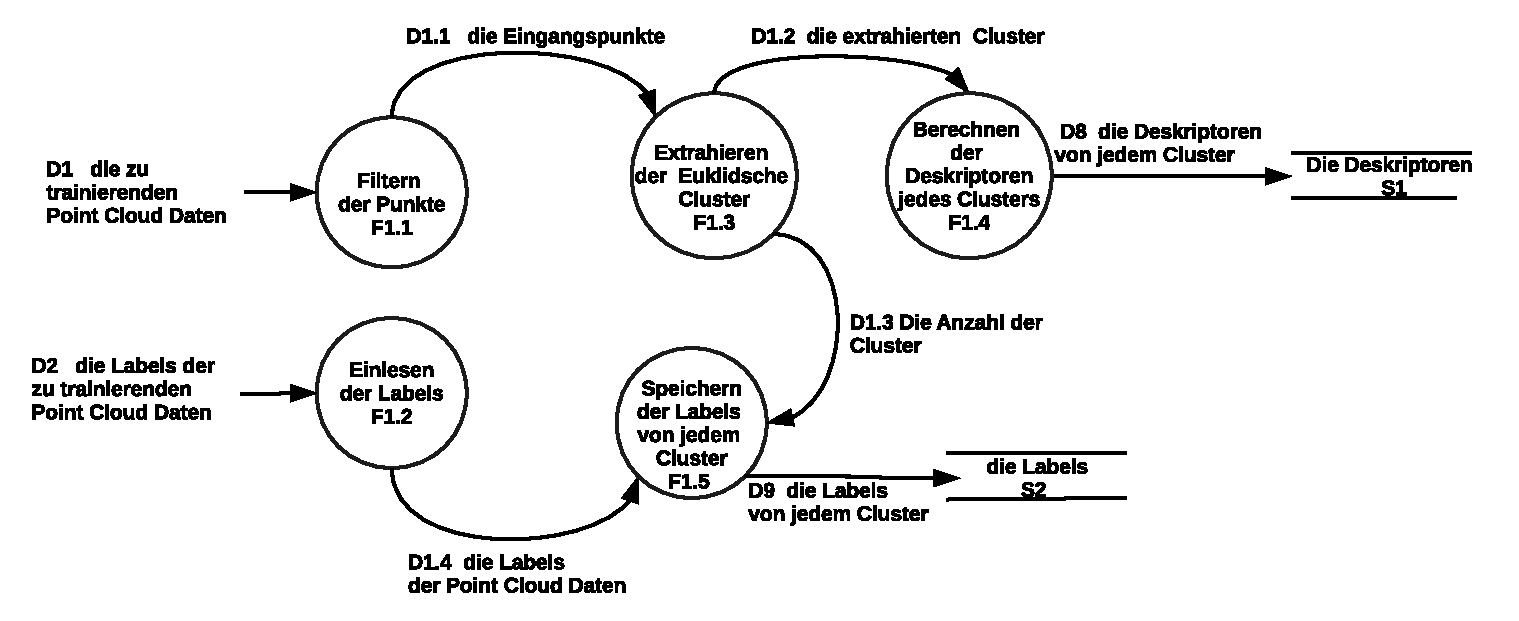
\includegraphics[width=1.0\textwidth]{example_files/log/DE2F1.eps}
    \caption{Datenflussdiagramm - Ebene 2 - Funktion 1}\label{fig:digit}
  \end{figure}
  
  
 \begin{table}[htb]
      \caption{Datenflussdiagramm - Ebene 2 - F1 - Funktionen}
       \centering
     \begin{tabular}{p{5.5cm}|p{8cm}}
      \hline
      \textbf{Funktion} & \textbf{Beschreibung}\\
      \hline
       F1.1  Filtern der Punkte & Die Punkte, die mit höhen Krümmung, sind gefiltert\\
      \hline
       F1.2  Einlesen der Labels & Die Labels der Point Clouds werden heruntergeladet.\\
      \hline
       F1.3  Extrahieren der Euklidsche Cluster &  Das Objekt wird mit bestimmten Euklidschen Distanz unterteilt\\
      \hline
       F1.4  Berechnen der Deskriptoren jedes Clusters &  Die Deskriptoren werden nach den unterteilten Clustern berechnet \\
       \hline
       F1.5  Speichern der Labels  von jedem Cluster &  Entsprechend der Nummer werden die Labels gespeichert \\
       \hline
       
    \end{tabular}
  \end{table}
  
  \begin{table}[htb]
    \caption{Datenflussdiagramm - Ebene 2 - F1 - Datenflüsse}
    \centering
    \begin{tabular}{p{5.5cm}|p{8cm}}
      \hline
      \textbf{Daten- oder Steuerfluss} & \textbf{Beschreibung}\\
      \hline
       D1.1 die Einganspunkte & die Punkte in der PointCloud nach dem Filtern\\
      \hline
       D1.2  die extrahierten Cluster  &  die unterteilten Cluster\\
      \hline
       D1.3 Die Anzahl der Cluster  &  Die Anzahl der Cluster der existierenden Cluster\\
      \hline 
       D1.4 die Labels der Point Cloud Daten &  Die Labels von jeder PointCloud  \\
      \hline
        
    \end{tabular}
  \end{table}
  
  
  


%%%%%%%%%%%%%%%%%%%%%%%%%%%%%%%%%%%%%%%%%%%%%%%%%
\subsection{Datenflussdiagramm - Ebene 2 - Funktion 3}

Die Abbildung 2.4 stellt die Dekomposition der Funktion: F3 dar. Die Tabellen
2.8 und 2.9 beschreiben die enthaltenen Subfunktionen und Datenflüsse.

\begin{figure}[h]
    \centering
    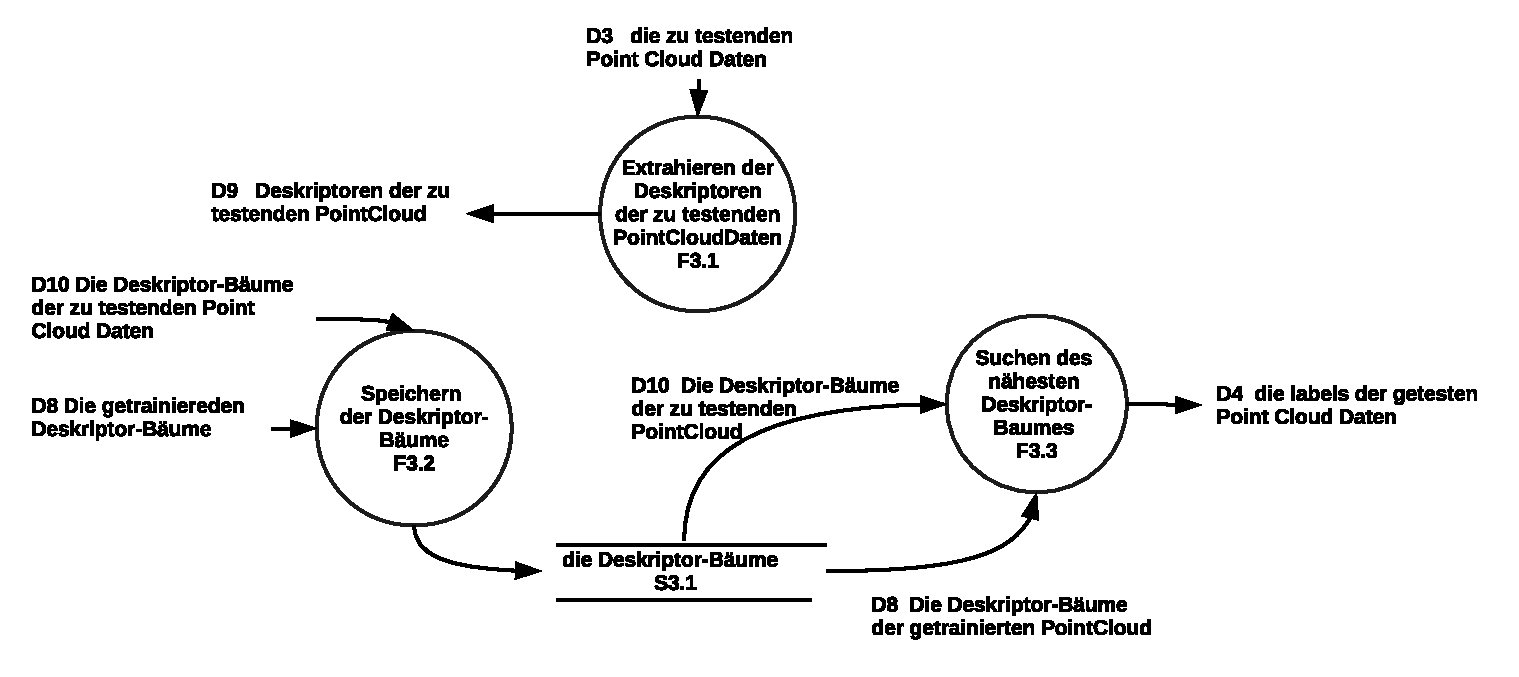
\includegraphics[width=1.0\textwidth]{example_files/log/DE2F3.eps}
    \caption{Datenflussdiagramm - Ebene 2 - Funktion 3}\label{fig:digit}
  \end{figure}
  
  
  
  \begin{table}[htb]
      \caption{Datenflussdiagramm - Ebene 2 -F3 - Funktionen}
       \centering
     \begin{tabular}{p{6.3cm}|p{8cm}}
      \hline
      \textbf{Funktion} & \textbf{Beschreibung}\\
      \hline
       F3.1 Extrahieren der Deskriptoren der zu testenden PointCloudDaten & Die Deskriptoren der Point-Cloud werden als Testdaten berechnet. \\
      \hline
       F3.2  Speichern  der Deskriptor-Bäume  &  Die erzäugten Deskriptorbäume werden gespeichert \\
      \hline
       F3.3 Suchen des nähesten Deskriptor-Baumes  & Die nähsten Deskriptorbäume werden in dem gespeicherten und trainierten Baum gesucht.\\
      \hline
       
       
    \end{tabular}
  \end{table}
  

%%%%%%%%%%%%%%%%%%%%%%%%%%%%%%%%%%%%%%%%%%%%%%%%%
\subsection{Datenflussdiagramm - Ebene 2 - Funktion 4}

\begin{figure}[h]
    \centering
    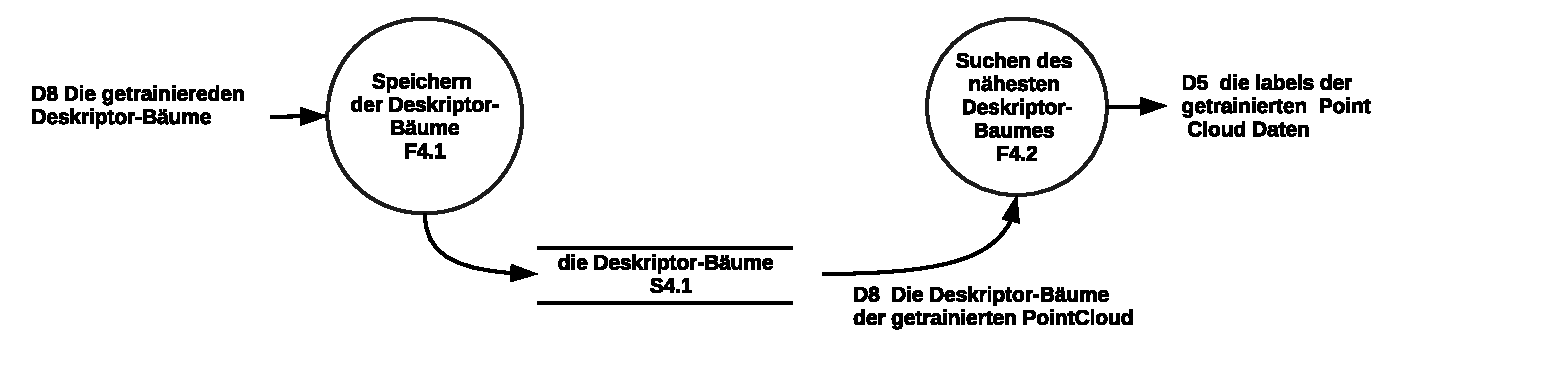
\includegraphics[width=0.95\textwidth]{example_files/log/DE2F4.eps}
    \caption{Datenflussdiagramm - Ebene 2 - Funktion 4}\label{fig:digit}
  \end{figure}



\begin{table}[htb]
    \caption{Datenflussdiagramm - Ebene 2 - F4 - Funktionen}
     \centering
   \begin{tabular}{p{6.3cm}|p{8cm}}
    \hline
    \textbf{Funktion} & \textbf{Beschreibung}\\
    \hline
     F4.1   Speichern  der Deskriptor-Bäume & Die erzäugten Deskriptorbäume werden gespeichert\\
    \hline
     F4.2   Suchen des nähesten Deskriptor-Baumes  &Die nähsten Deskriptorbäume werden in dem gespeicherten und trainierten Baum gesucht. \\
    \hline
    
  \end{tabular}
\end{table}







